\documentclass{article}

\usepackage[english]{babel}
\usepackage[utf8]{inputenc}
% Set page size and margins
% Replace `letterpaper' with `a4paper' for UK/EU standard size
\usepackage[a4paper]{geometry}
\usepackage{mathptmx}
% Useful packages
\usepackage{amsmath}
\usepackage{graphicx}
\usepackage{minted}
\usepackage[colorlinks=true, allcolors=blue]{hyperref}
\usepackage{url}

\title{COMP321 Information System Implementation 
Final Report}
\author{King P-19-0955-4,
Steve P-19-0832-6,
Stephen P-19-0836-4,\\
Freddie P-19-0830-7,
Jane P-19-0834-5}

\begin{document}
\maketitle

% \tableofcontents

\section{Introduction}

How often do you usually shop online? In the last decade, an explosive growth of online shopping has rapidly replaced people’s habit of shopping in real markets. Since it represents a more economic and convenient approach to purchasing items, the online shopping markets with different targets also flood up in these years\cite{1.1}. Nowadays, it is not how to shop online but which online shopping mall is worth a try is the essential problem for users. Therefore, this report will focus on analyzing the performance of the self-developed mobile shopping market and explain the practicability and convenience of this conceptual online mobile market.
\subsection{Overview}

Over years of technology advancement, it has created countless opportunities with endless resources which have practically changed the way things are rolled. There are countless examples of technology creating a better life. Among them, with the popularity of various e-commerce platforms, shopping is never bound by time and space, and people are gradually getting used to this way of shopping on their mobile phones without leaving home. In addition, vendors cost much less to monitor commodity transmissions and related works. 
\\\\
Our developer team will design a conceptual mobile shopping market named Open Mall based on this trend, which carries our understanding of technology convenience. It is maintained to provide an easy, convenient, secure, and user-friendly online shopping platform. Besides, it bases on a business-to-customer model. Therefore, people can register to be a customer in the online shopping market to purchase items\cite{1.2}. 
In this shopping market, the shopping process will be simple and easy, and customers can purchase whatever they want especially electronic devices and sneakers efficiently without distance bound. On the other hand, a vendor-side view will also be created for commodity distribution and shopping process monitoring.
\\\\
This project report provides the details on all the work within the development of the online mobile market system. Vendors present their products in a way that is convenient for customers to choose and purchase. Additionally, the process design of purchase order tracking and purchase order processing is provided.

\subsection{Objectives}
The main objective of this project is to develop a mobile online market that allows customers to do shopping at the front-end of the mall, browse and select desired products. First, functions like paging, filtering, searching and price sorting should be provided to help customers to do shopping more convenient. Then a shopping cart feature should be realized to place orders. Besides, the vendor would maintain a product catalog in the shopping mall. purchase order should be tracked and processed in stage by the vendor as well. 
\\\\
Notably, this report is geared to the audiences which include website administrators, mobile application developers, and web maintainers. 
\\\\
This report is organized as follows: Chapter 2 introduces the background of online shopping websites. Chapter 3 presents our design approaches. Chapter 4 shows the implementation details. Chapter 5 is about the outcome of our project and some discussion on it. Chapter 6 includes the conclusion and ideas for future work.

\section{Background and Related work}

Electronic commerce is the activity of having online transactions between buyers and vendors. This chapter explains the background and related work. In the background section, the common features of these e-commerce platforms are elucidated. In addition, the comparison between several existing websites or e-commerce packages and our works is delineated in the related word section.

\subsection{Background}
E-commerce (electronic commerce) is defined as the buying and selling of goods and services, or the transmitting of funds or data, over an electronic network, primarily the internet. E-commerce can be categorized into three different types, basically – Business-to-Business (B2B), Business-to-Consumer (B2C), and Business processes. Two other categories are also known: Consumer-to-Consumer (C2C), which is included in the B2C category, and Business-to-Government (B2G), which is included in B2B discussions. \cite{2.1}
\\\\
In this context, various e-commerce platforms have emerged. Despite their differences, there are some general features in these platforms. Since the platforms are mainly used to serve two main types of users – customers and vendors, these common features can be divided into two parts.
\\\\
In terms of features for customers, these features are to achieve a pleasant experience to select and purchase goods. Specifically, individual accounts are always provided to the customers so that they can have their purchases records. In addition, to make customers find what they want to buy quickly, a search function is offered. Similarly, some filters are given so that the customers can narrow the scope of goods by price, brands, or other aspects. Moreover, the basic information is imparted for each good listed in the product list. Furthermore, the shopping cart is provided for customers to pay for many goods together. Last but not least, online payment is allowed.
\\\\
Moving on to the features for vendors, these features are to make vendors manage the goods and purchase orders easily. To be more specific, individual accounts with specific authorities for vendors are offered. In addition, the products can be created, read, updated, and deleted by vendors. Finally, the purchase orders can be listed and changed.

\subsection{E-commerce situation in Macao and Mainland of China}
The number of local households using the Internet in 2019 increased by 6,900 year-on-year to 182,300, accounting for 92.3 percent of all households.  Internet users aged 3 and above totaled 554,000, up by 5 percent year-on-year. The Internet penetration rate for members of the population aged 35 to 44 and 25 to 34 reached 98.6 percent and 98.0 percent, respectively; and 69 percent of the population aged 55 and above used the Internet, an increase of 5.3 percentage points. Most of those surveyed reported that they use the Internet for communication and online entertainment. Online shoppers rose 30 percent to 123,900 in 2019.
\\\\
From these data, we can easily know the situation in Macao. The situation in the mainland of China is also very impressive. The E-commerce revenue growth trend displays positive relationship with online shopping people very well as Figure \ref{fig:Macau E-commerce}.
\begin{figure}[!htp]
    \centering
    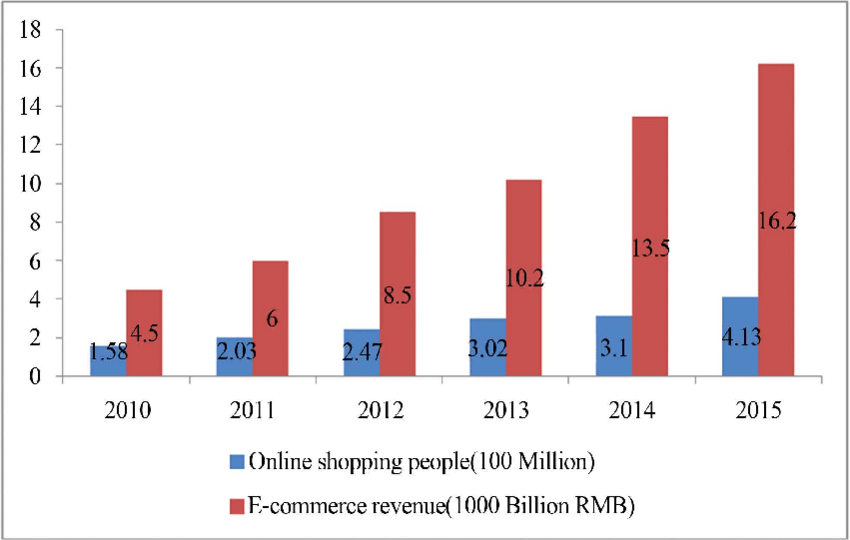
\includegraphics[width=0.6\textwidth]{Macau E-commerce.png}
    \caption{\label{fig:Macau E-commerce}Situation of Macau E-commerce}
\end{figure}

\section{System Design}

In this chapter, we describe our database structure through the ER diagram and explain our design decisions. Besides, we will present the activity diagram to illustrate the interaction of the customers with our system.

\subsection{Data Modelling}
In this section, ER diagram and data dictionary, as well as the design concepts will be presented. 
\\\\
Figure \ref{fig:ER Diagram} shows the entities \verb|(account, address, order, product, purchase, and shopping_cart)| and the relationships among them in our online shopping system.
\begin{figure}[!htp]
    \centering
    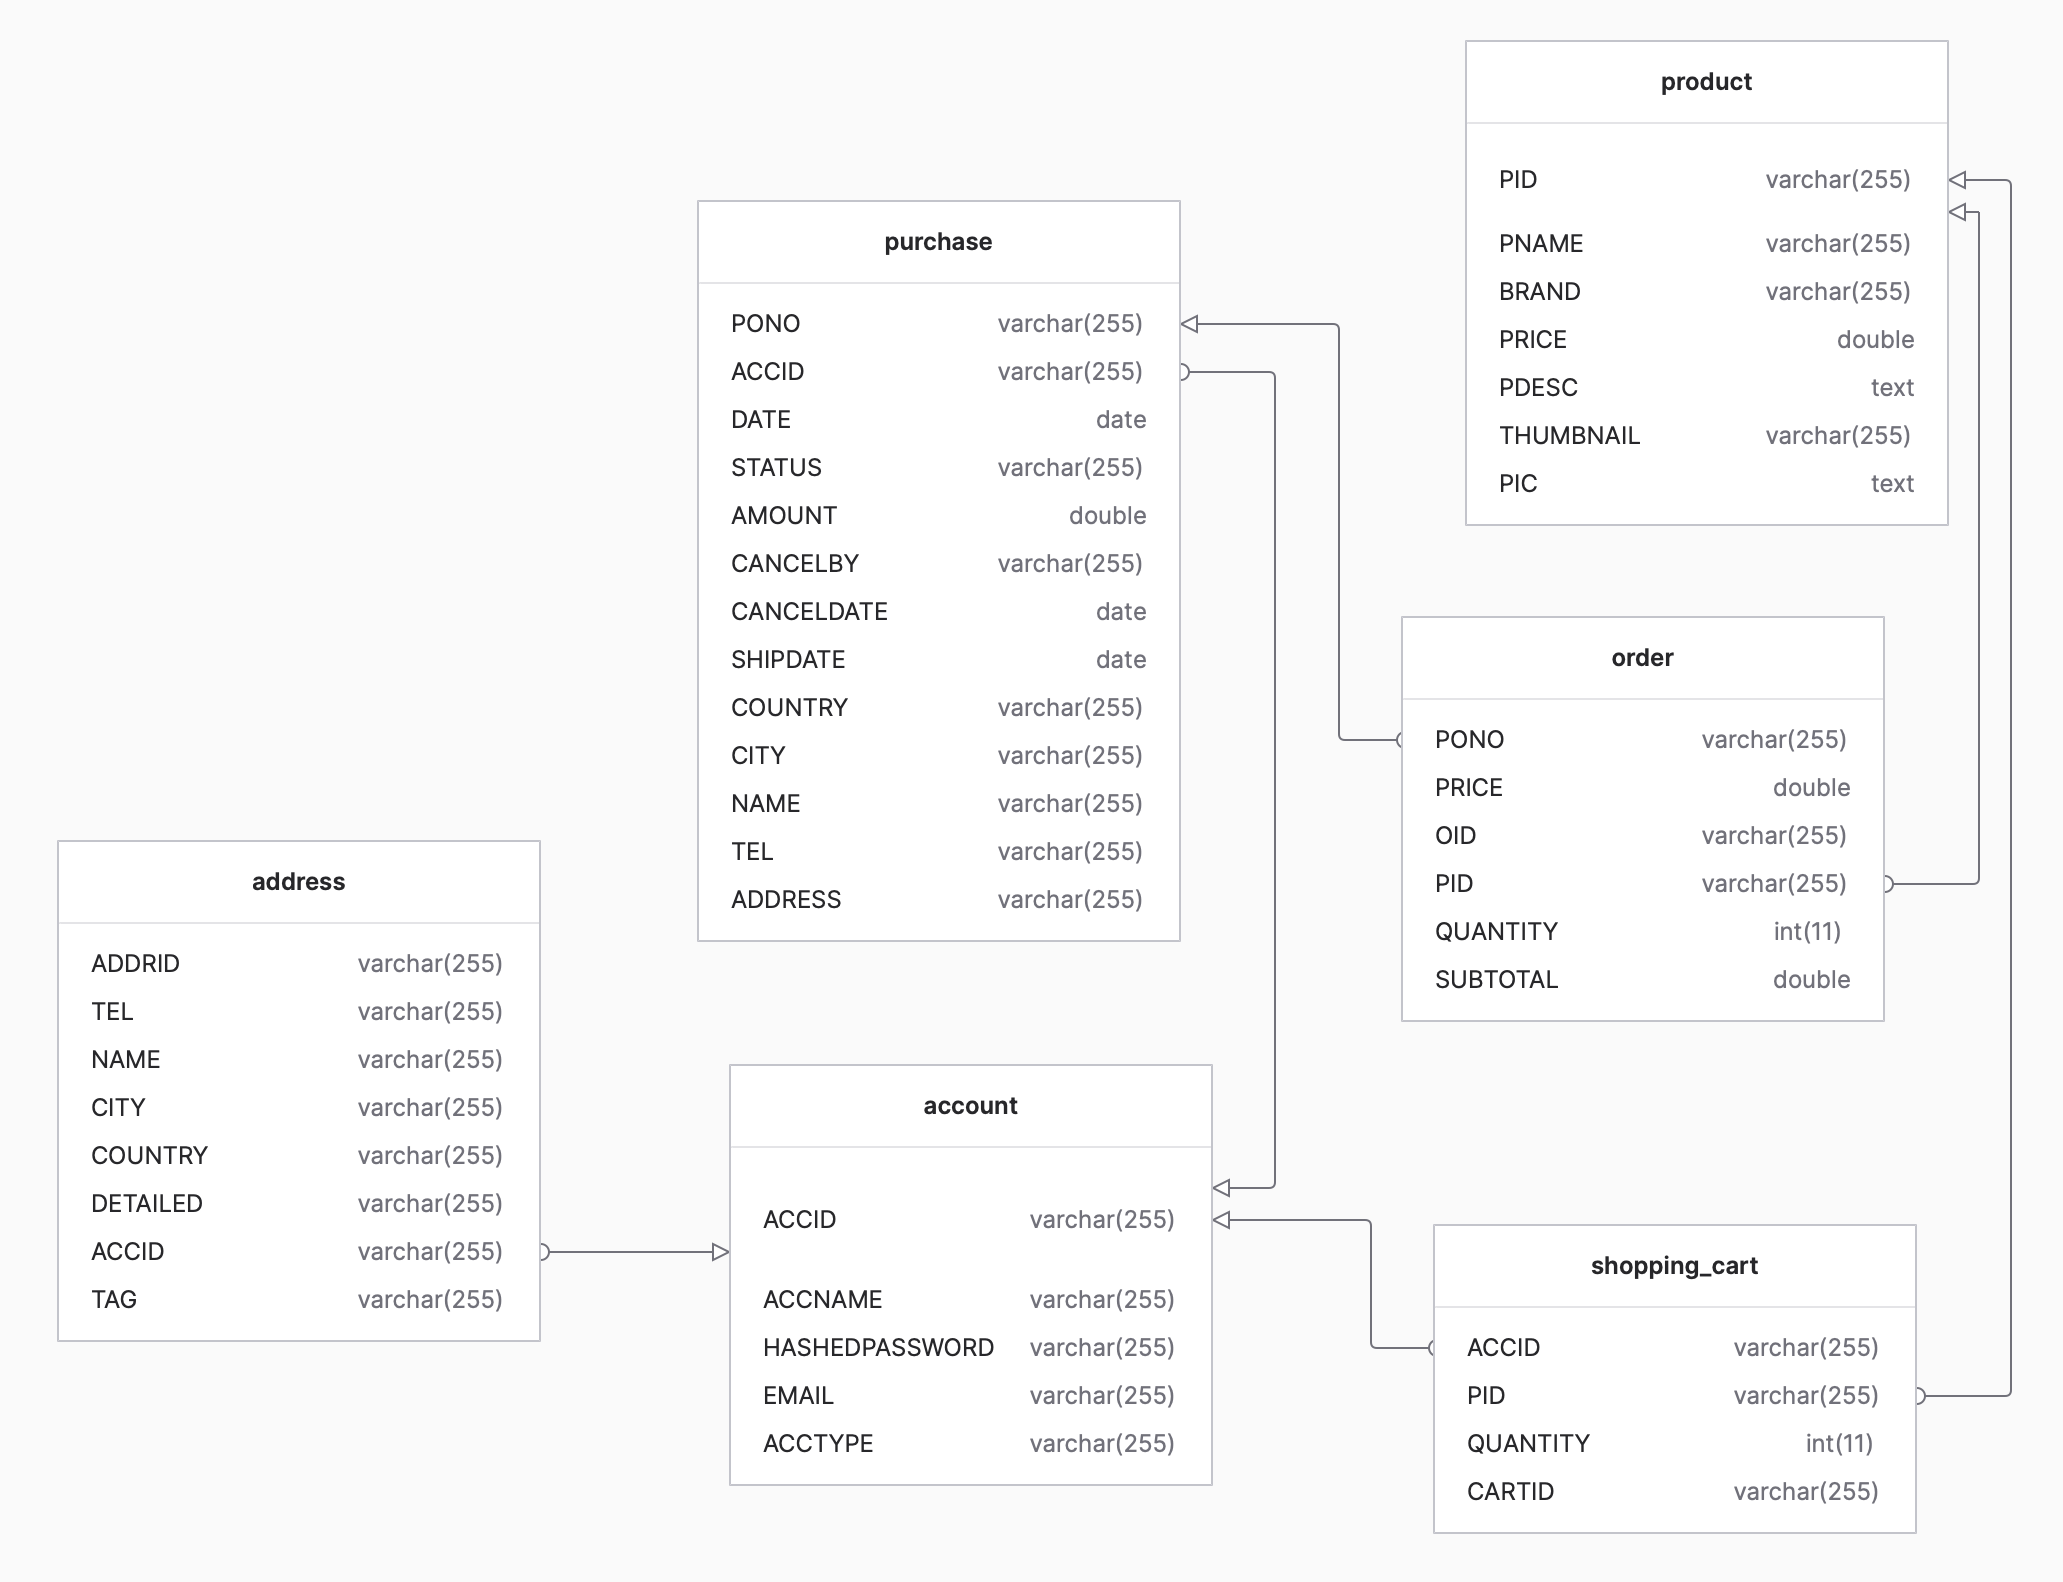
\includegraphics[width=0.7\textwidth]{ER Diagram.png}
    \caption{\label{fig:ER Diagram}ER Diagram}
\end{figure}
\\\\
The entity account represents the users registered in the system with account ID, account name, password in hash style, and email address. The attribute \verb|ACCTYPE| indicates the account type of the current user such as admin, vendor, or customer. 
\\\\
Considering multiple addresses are reasonable to exist under one user account, we use the entity address to deal with this scenario.
\\\\
The entity product records all the information about the goods, such as its unique product ID, product name, brand, the list unit price, all the related pictures, and a detailed description of the goods. Among them, the thumbnail image indicates the image to be shown on the store page, while all the pictures in the \verb|PIC| field will be displayed only on the product detail page
\\\\
The entity shopping\_cart simply stores the products that the users are interested in buying. The quantity will be stored as well. Considering all the calculation about the price will be recorded in the order once created, the amount will not be recorded in this field due to reduce the pressure of change on services.
\\\\
The entity purchase represents an order purchased by customers on the website with order number \verb|PONO|. This purchase list stores the account that creates this order, the date of purchase, the current order status, and the shipping date if the goods have been shipped. Information about when and by whom the order is canceled will also be recorded if it occurs. Each purchase contains one or more products.
\\\\
The entity order represents each of the individual products purchased. It stores the purchase price instead of the current list price and the subtotal calculated by the purchase unit price times quantity. 

\begin{verbatim}
Account (ACCID, ACCNAME, HASHEDPASSWORD, EMAIL, ACCTYPE)
Address (ADDID, ACCID, TEL, NAME, CITY, COUNTRY, DETAILED, TAG)
Product (PID, PNAME, BRAND, PRICE, PDESC, TRUMBNAIL, PIC)
Shopping Cart (CARTID, ACCID, PID, QUANTITY)
Purchase (PONO, ACCID, date, STATUS, AMOUNT, CANCELBY, CANCELdate, SHIPdate)
Order(OID, PONO, PID, PRICE, QUANTITY, SUBTOTAL)
\end{verbatim}

Figure \ref{fig:Data Dictionary} shows the data dictionary of all the entities and the related attributes of our system.
\begin{figure}[!htp]
    \centering
    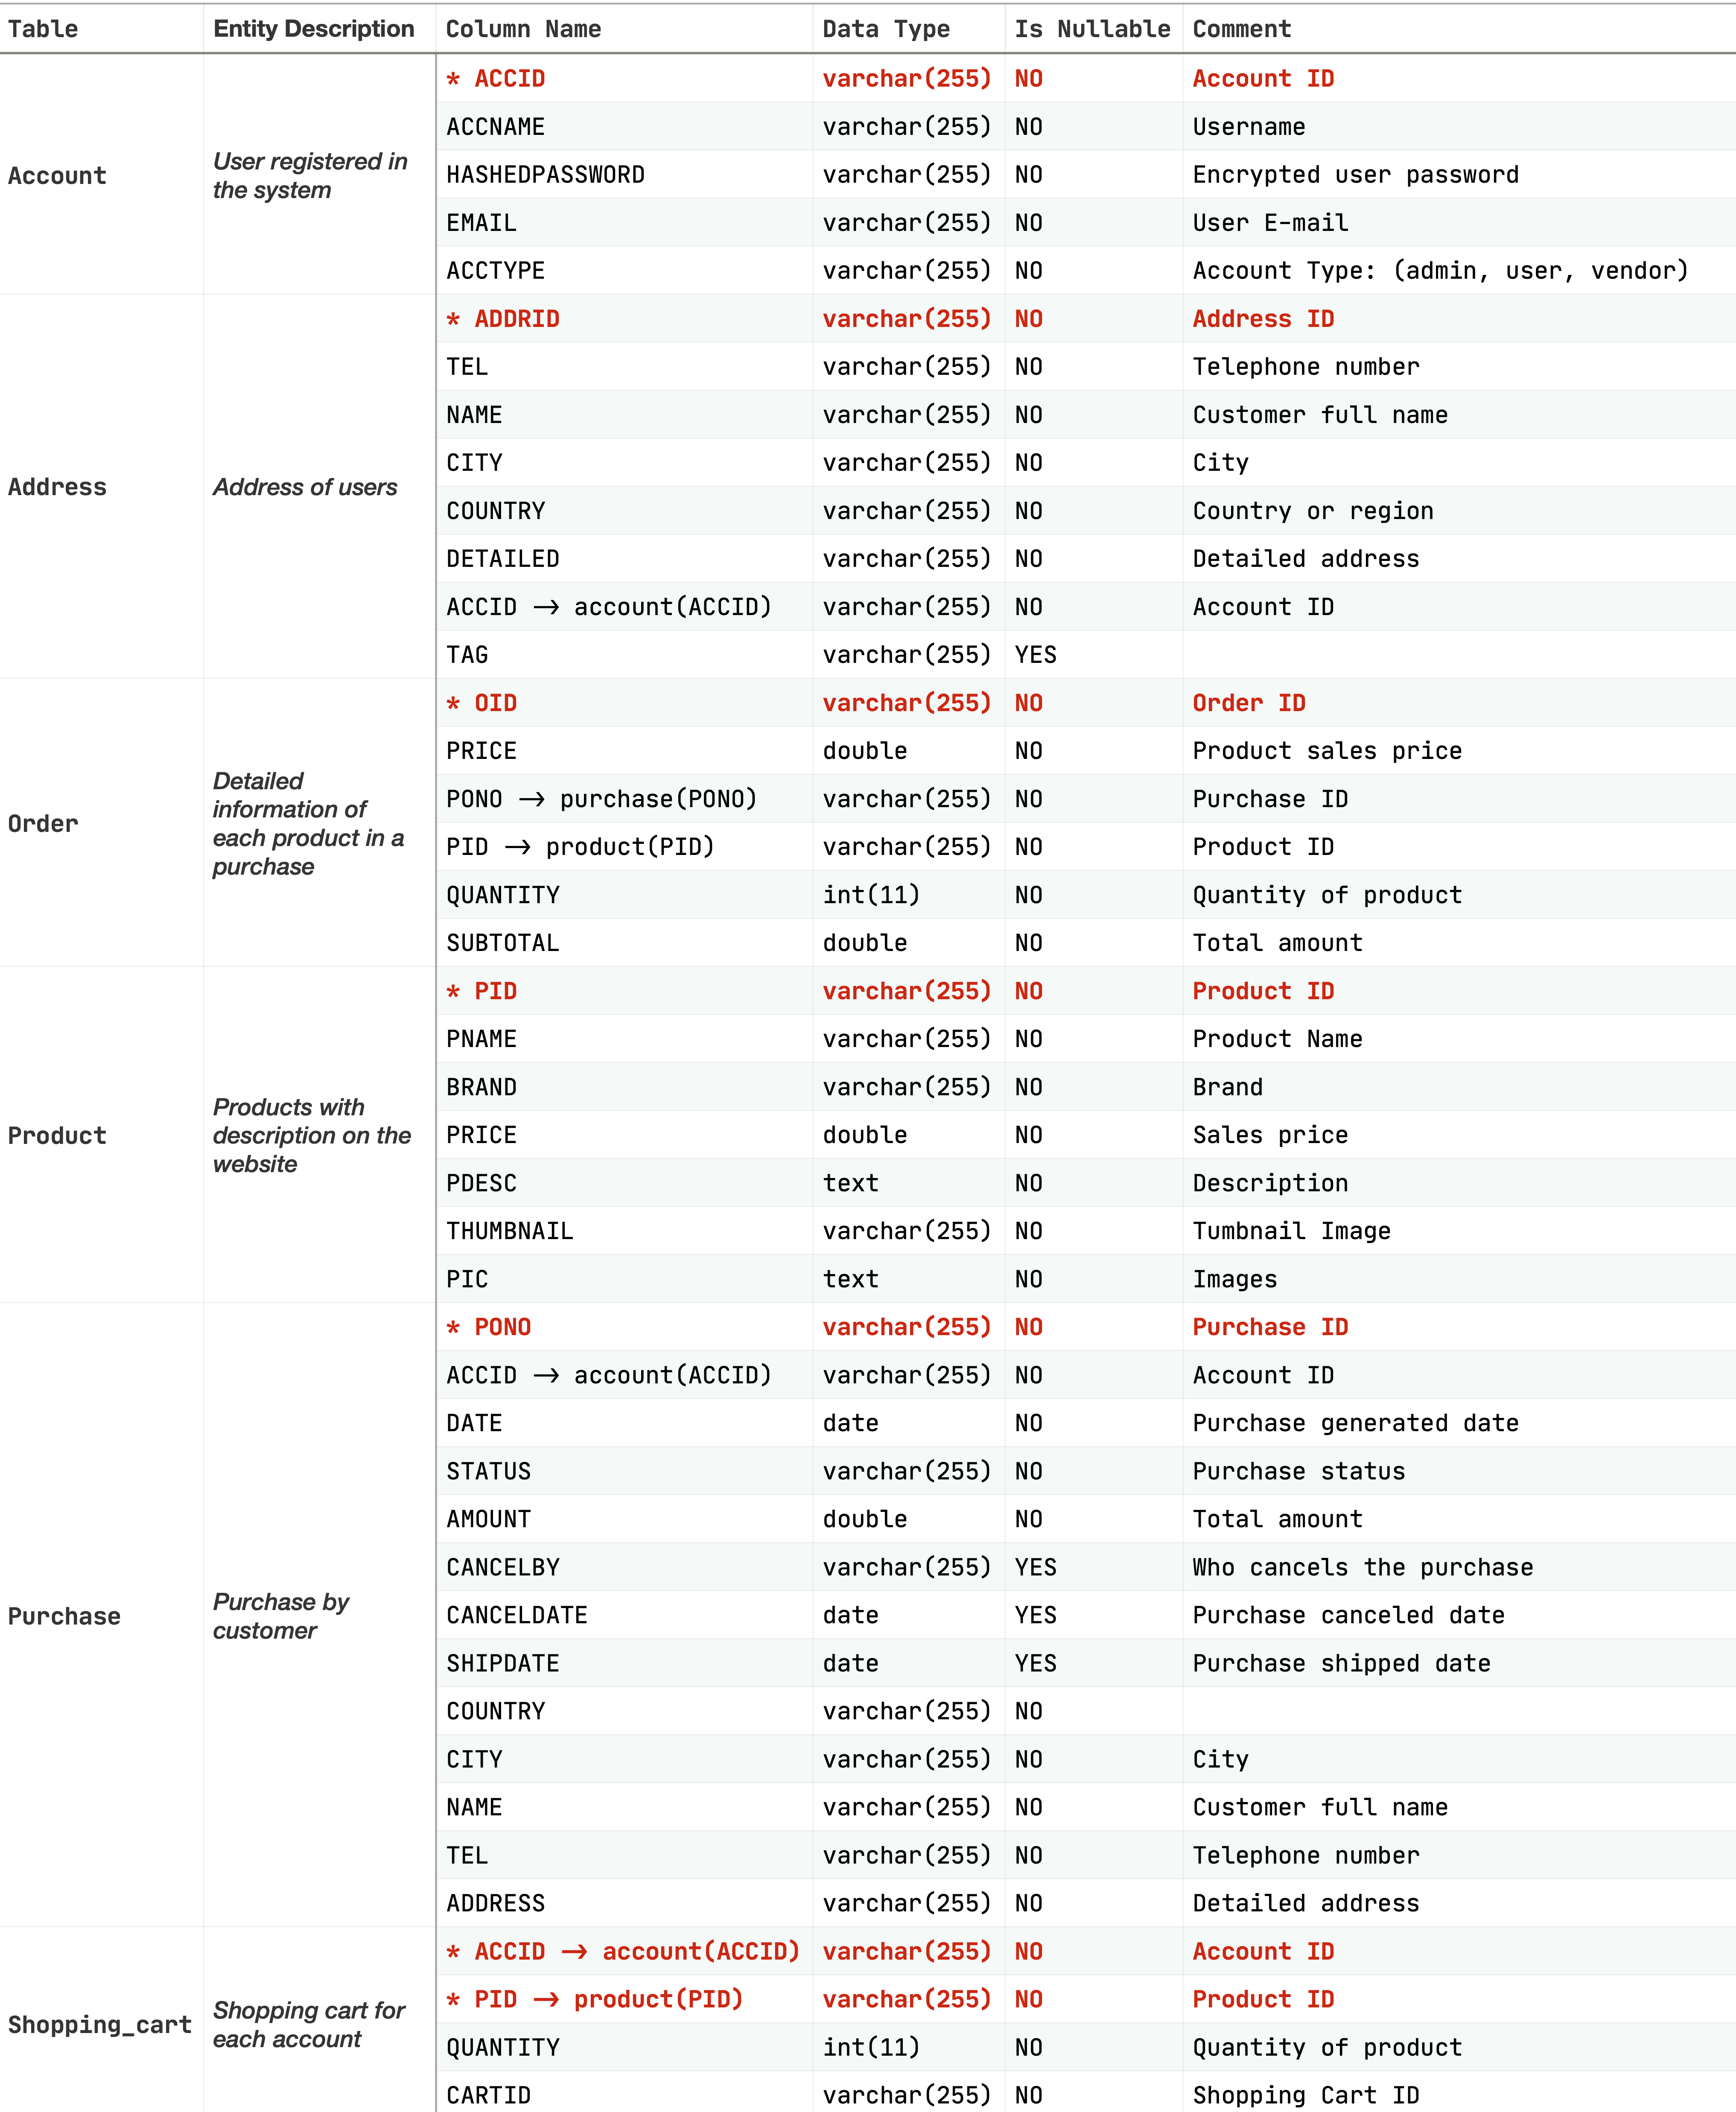
\includegraphics[width=1\textwidth]{Data Dictionary.png}
    \caption{\label{fig:Data Dictionary}Data Dictionary}
\end{figure}

\subsection{Dynamic Modelling}
In this section, we address the interaction between the users and our system in the format of an activity diagram.
\\\\
Figure \ref{fig:Activity Diagram} depicts the control flow start that shows the various decisions paths customers can choose and enter. Customers can only browse the product list and product detail page before login. While with the legal customer account, users are permitted to add desired items into the shopping cart. After checking the commodities and the quantity setting, the users can create an order to purchase goods in the meantime the shopping cart would be emptied. All the order status following can be monitored by the user. Other operations on the order like deleting before the goods are shipped can be allowed.  Besides, all of the order histories are admitted to be checked. Additionally, an accounted user can manage his/her setting such as address management and password setting. 
\begin{figure}[!htp]
    \centering
    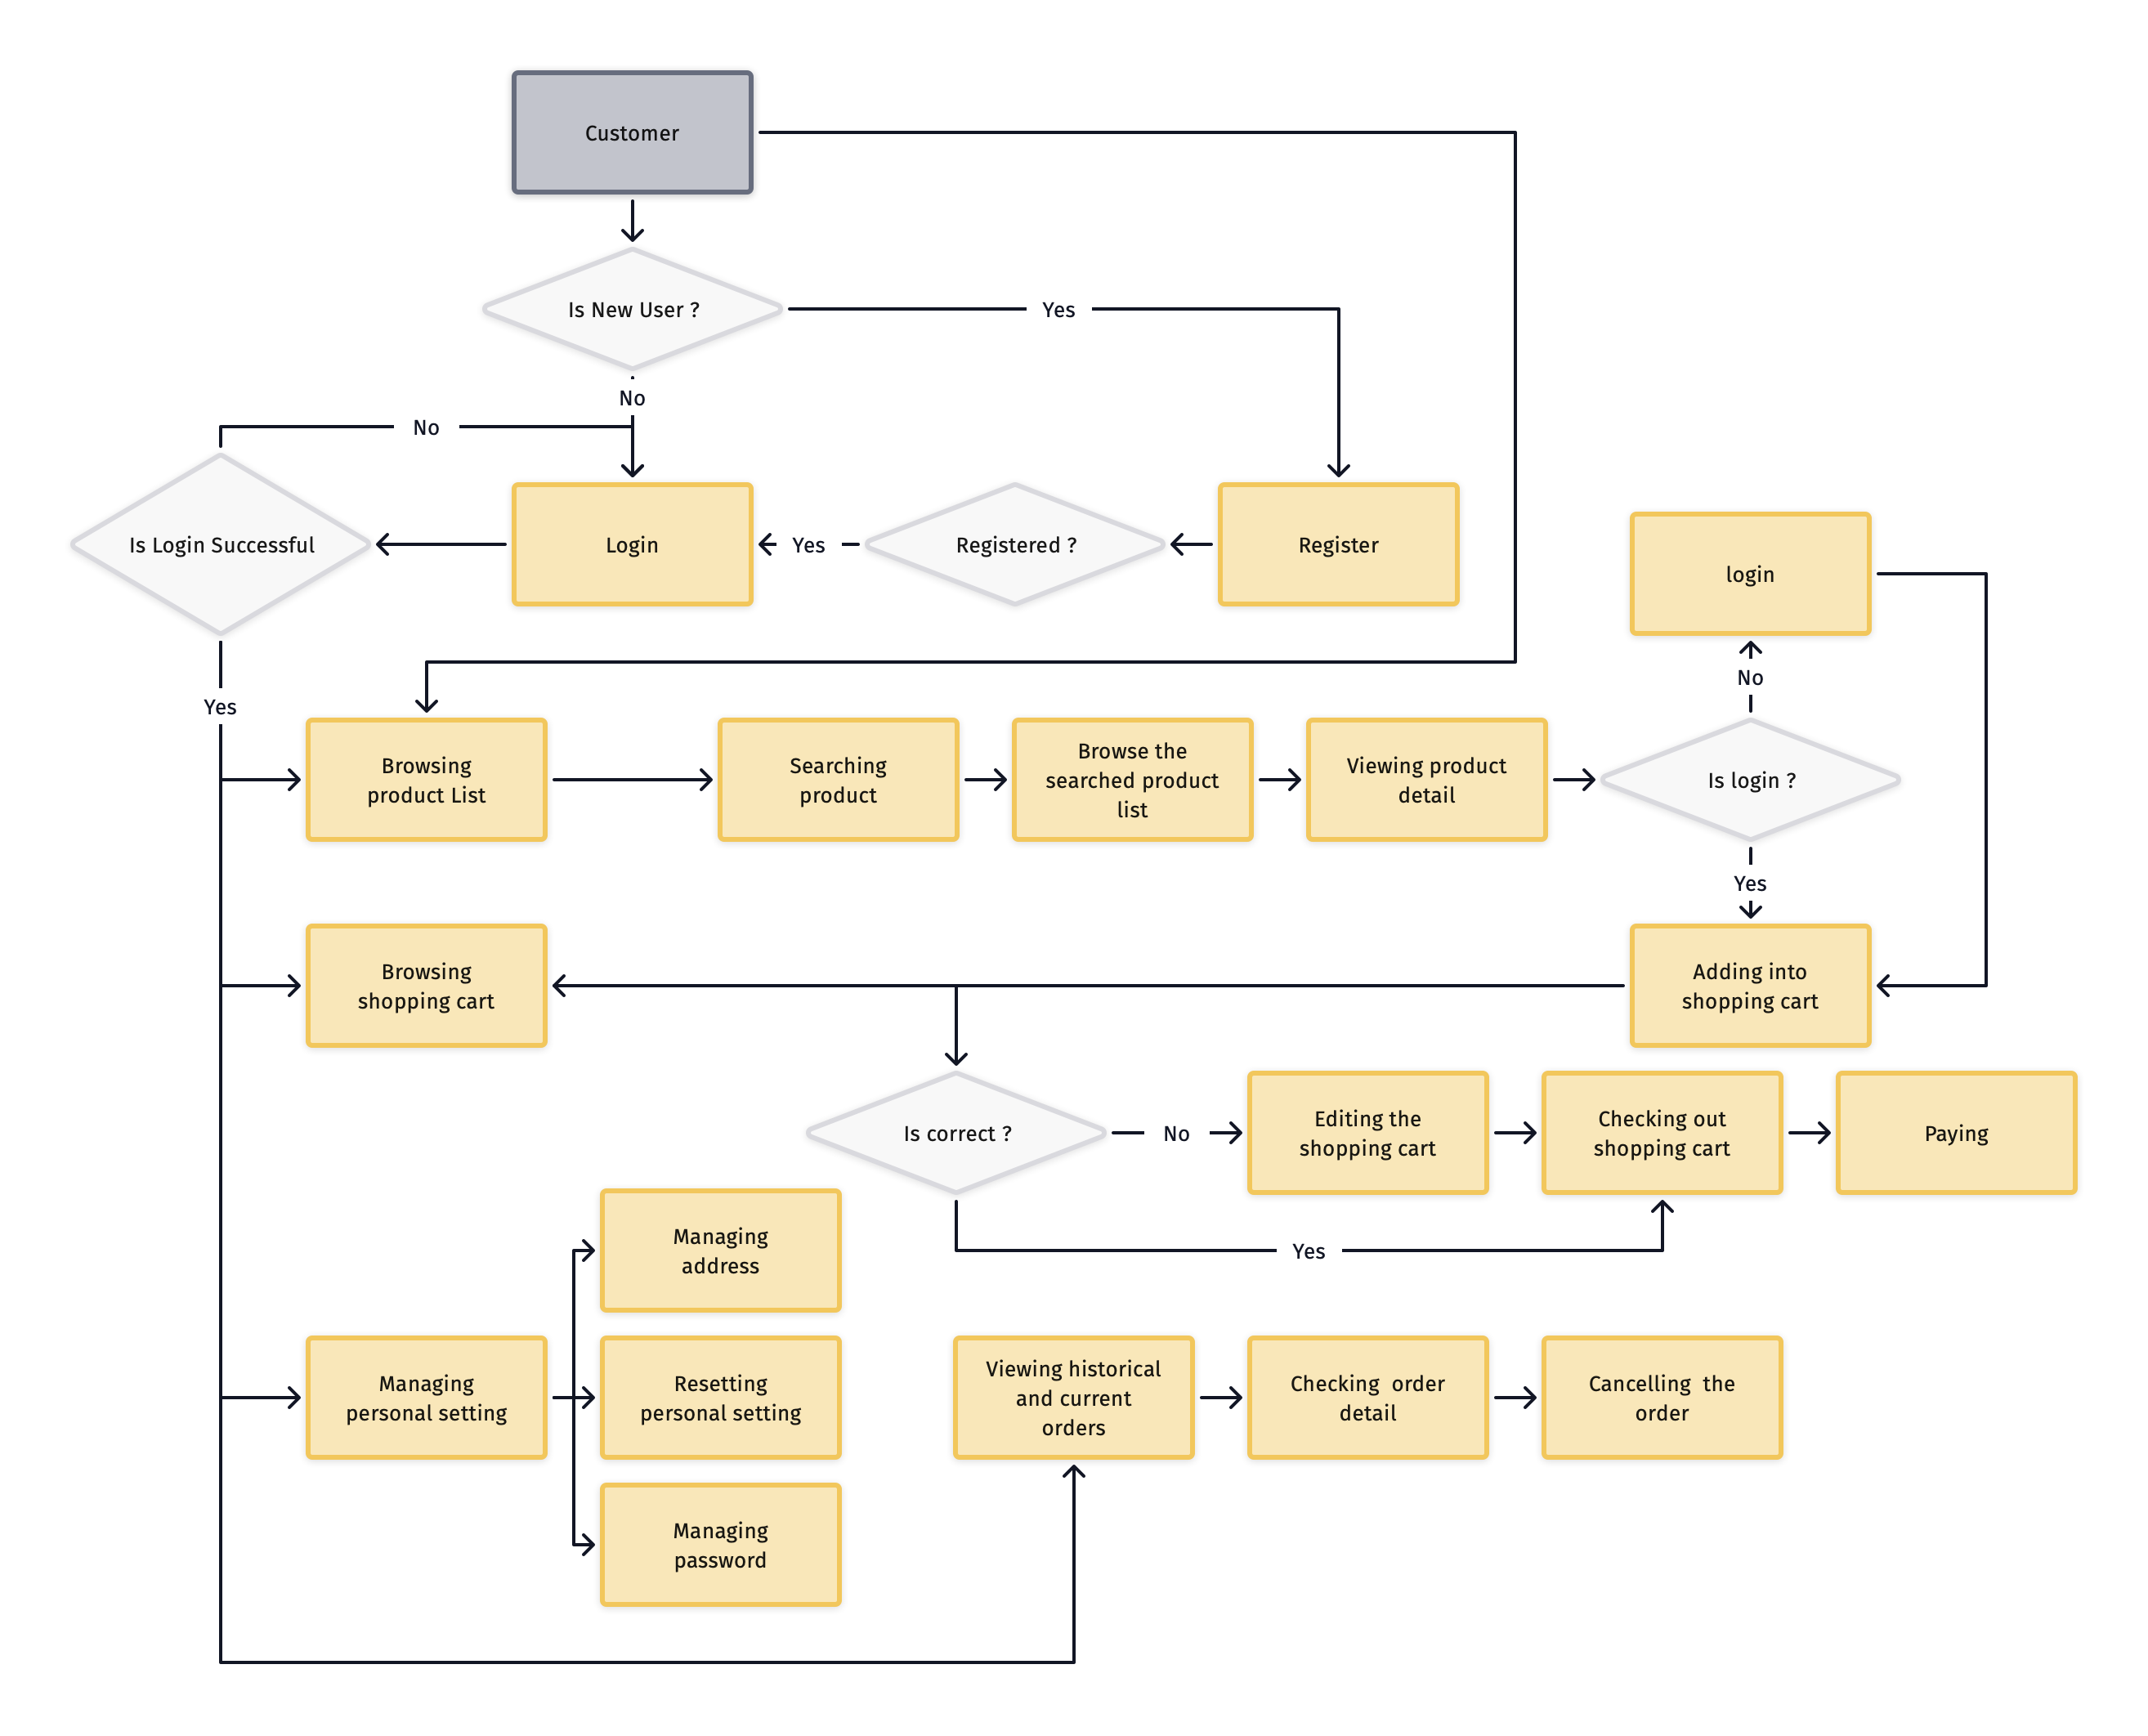
\includegraphics[width=0.9\textwidth]{Activity Diagram.png}
    \caption{\label{fig:Activity Diagram}Activity Diagram}
\end{figure}

\section{System Implementation}

In this section, the architectural implementation will be introduced. In brief, we implement OpenMall with the technical stack of separation of front-end and back-end, which is a famous solution in modern web applications. Moreover, this solution is leading the era of extensive front-end. Instead of the traditional web framework rendering the webpage on the webserver, the modern approach enables the effective exchange of data via \verb|JSON| and other data-interchange formats. The rendering process of the webpage is transferred to the client's computer, which substantially saves the resources in the webserver and the transferring bandwidth.

\subsection{Architecture}

OpenMall involves the separation of the front-end and back-end and the client App. Thus, the architecture is mainly in three parts, namely front-end, back-end, and client App.

\subsubsection{Front-end}

We adopted Vue.js 3.0 to implement the Single Page Application (SPA) \cite{spa} approach in front-end design. Different from the widely used version 2.0 of Vue.js, we implemented a large portion of code by using the new feature in Vue.js 3.0 like setup scripts. The lack of documentation and community support makes the implementation challengable. In addition, fewer plugins supported Vue.js 3.0 than Vue.js 2.0, which means we need to implement many infrastructures from scratch. Nevertheless, we successfully implemented our OpenMall e-commerce platform, and it meets all of the functional requirements.
\\\\
The visual design of OpenMall is implemented using Tailwind CSS. Raw and complex CSS codes have been avoided. Tailwind CSS significantly reduces the difficulty in UI and UX design. Moreover, the mobile-first design of Tailwind CSS enables effortless implementation in porting the mobile App.
\\\\
To communicate with the back-end. We coupled Axios in the front-end Vue.js scripts. Axios as an alternative to the original \verb|fetch| in JavaScript. It provided more function parameters and a more convenient passing of parameters with \verb|POST| requests. Detailed implementation of data communication will be introduced in the back-end section later.

\subsubsection{Back-end}

The back-end implementation includes the API server, Webserver, database. We considered FastAPI as an ideal API server that is minimally designed and can implement with Python. The Nginx Web server is for distributing web applications (front-end distribution). For the database, the open-source MariaDB is a perfect choice. This database management system balances performance and scalability. Then, we deployed the API server, Web server, and database on a single server. That server is an Elastic Hosting provided by Alibaba cloud. In deployment, we adopted a containerization solution by using Docker. Both the Nginx Webserver and MariaDB are running in two Docker containers.
\\\\
FastAPI is an API server implemented with Python. It has very high performance. To cooperate with the front-end technical stack of Vue.js, FastAPI is an appropriate choice. The FastAPI server comes with the front-end API documentation. Thus, the front-end JavaScript developer can play around with the API documentation to send requests to the back-end, which favors them in debugging and testing APIs.
\\\\
The webserver we used here is for distributing static files which need to send to the client browser. The static file is an HTML file. It is built by the Vite builder. We will introduce the static file in the next section of Integration of Front-end and Back-end. Back to the webserver, we adopted Nginx. It was the second-most widely used web server across all "active" sites and for the top million busiest sites. Moreover, it implemented the WSGI standard. Although in our project, the webserver is just for content distribution. The Nginx server is also a good choice.
\\\\
The most important part of the back-end is the database. We deployed the MariaDB at the beginning of our project on the cloud. We maintained a unique copy of the data. The cloud-based database makes the further development of different computers of our members easier. The choice of database is MariaDB, which is the community-supported version of MySQL. It has excellent performance and a variety of community support. As for the core part of our project, it is essential to be consistent. Especially for the table schema. If there is inconsistency, the development and debugging process will be in big trouble. In the meanwhile, alternating the table schema during the development process is fatal. In the Data Modelling process, there was a fault that we failed to consider the changes in user addresses. Then we designed the \verb|Purchase| table with only the user address ID foreign key. Finally, we noticed the failure of the design. So we need to rewrite several lines of code. And this led to several bugs in many lines of code related to business logic. Hence, we need to consider all of the situations in the data modeling process.

\subsection{Integration of Front-end and Back-end}

Apart from the traditional webpage. The server renders all of the user data of a specific user and sends the rendered webpage to the client browser. Modern web applications adopted the separation of front-end and back-end methods similar to mobile applications. That is, when a client user requests the web application, the static file server (we implemented using Nginx) sends a webpage (application more accurately) to the client browser. Till now, the client browser can run the web application locally without fetching data. If the scenario is data-driven, like our OpenMall project, the web application should have data communication with the API server. The web application works with fetching and sending data from or to the API server. And the process of data communication using EDI is mainly the integration.

\subsubsection{Resolving the issue of Cross-origin resource sharing}

JavaScript and web programming have grown by leaps and bounds over the years, but the same-origin policy still remains. This prevents JavaScript from making requests across domain boundaries and has spawned various hacks for making cross-domain requests. Corss-origin resource sharing (CORS)\cite{cors} introduces a standard mechanism that can be used by all browsers for implementing cross-domain requests. The spec defines a set of headers that allow the browser and server to communicate about which requests are (and are not) allowed. When the front-end web application communicates with the back-end, CORS restricts the communication process. Thus, we need to specify the request header and tell the server and client browser that it should be allowed for all of the essential sites when using our system.
\\\\
To resolve the CORS issue. We need to configure the FastAPI using middleware. To achieve this, the backend must have a list of "allowed origins". The core code is attached.
\begin{minted}{python}
from fastapi import FastAPI
from fastapi.middleware.cors import CORSMiddleware

app = FastAPI()

origins = [
    "http://localhost",
    "http://localhost:8080",
]

app.add_middleware(
    CORSMiddleware,
    allow_origins=origins,
    allow_credentials=True,
    allow_methods=["*"],
    allow_headers=["*"],
)
\end{minted}


\subsection{Containerization deployment}

\subsection{Product Search and Detailed Display}

\subsection{Image Storage and Handling}

\subsection{Password Security}

\subsection{Purchase Order Processing}

\subsection{Concurrency Control}

\subsection{Persist User Status in separation of front-end and back-end}

\section{Result and Discussion}

\subsection{Project Outcome}

\subsection{Testing and System Evaluation}


\section{Conclusion and Further Work}
In this project, the Open Mall application with products browsing, maintaining,  placing, and processing purchase orders for multitype of users has been successfully implemented. Vue.js was used to build the front-end view and we implement the back-end API based on FastAPI. MariaDB was our database management system to build and maintain our database. Finally, Xcode SDK was used to port the web mall to a mobile application.
\\\\
For the front-end interfaces for users, the user login page,  product list page, product detail page, shopping cart page, purchase tracking page, and purchase order detail page have been designed for customers. Meanwhile, the product catalog maintenance page and purchase order list page have been built for vendors. All the front-end layout and style designs of pages were based on HTML5 and Tailwind CSS. The front-end logic was implemented based on the Vue.js framework. We tested and verified the whole shopping process of users and the mall maintenance process of vendors by the method of the cognitive walkthrough after deployment.
\\\\
As for the back-end part, the APIs that handle front-end requests and invoke the required data of the database have been implemented. All the APIs were built by the Python-based FastAPI Framework. We used MariaDB to build the database and implement six entities: \verb|Account, Address, Product,| \verb|Shopping Cart, Purchase, Order|. Moreover, various SQL query statements and permissions of different users have been defined.
\\\\
When it comes to porting the Open Mall web to a mobile application. The front-end interfaces have been restructured by using the Xcode SDK to make them available for mobile devices. Simultaneously, Xcode SDK was used to the interactions between the Open Mall application and the operating system of Apple devices. 
\\\\
Inevitably, there are also limitations in the Open Mall project. First of all, Open Mall was a hybrid application, but not a native application. Therefore, the response time of the application is slightly slower than that of the native applications such as page load time. Secondly, logistics systems and payment gateways have not been integrated into the Open Mall application. What is more, the user’s community which allows users to make comments about the particular product and view evaluations from other users have not been implemented. Besides, the language system does not have supported for multi-language for the moment. 
\\\\
In the future, the Open Mall application will be updated to a native application for higher efficiency and response speed. A brand-new user community that supports users’ comments and communication in the form of pictures, text, and videos will be implemented. Additionally, the logistics system, payment gateways, and multi-language system will be tightly integrated into the Open Mall application. 

\bibliographystyle{abbrv}
\bibliography{reference}
\end{document}
